\chapter{Methodology}
\label{chp:methodology}

Now that the compositional models and the \gls{vcr} task were explored, this chapter will follow by going into detail about how the \gls{snmn} model was adapted to the \gls{vcr} dataset.
The details of how the dataset is prepared will be discussed first, going over any the extracting of image and text features, how these are processed, and any other data to be extracted.
The model adaptations performed will then follow, covering how the model will operate on the newly-generated data.
Finally, the experiments and how they were set up will be discussed.

\section{Data preparation}
\label{sec:data_preparation}

Before the model can begin to perform \gls{vqa} tasks, the required data must first be prepared into a format that will be understood by the model. The procedure below is followed across all datasets trained and tested on, with variations being made depending on the structure of the data.

The images are first pre-processed into a feature-set using a \acrshort{resnet}-152 model \cite{he_deep_2015} — pre-trained on the ImageNet\footnote{\url{https://www.image-net.org/}} dataset \cite{deng_imagenet_2009} — which outputs a 7x7x2048-dimension feature map of each image.

The question-answer pairs found in the dataset are processed after the images. For each question and answer sentence, the sentence is first collected into a single \gls{corpus} for later processing. The sentence is tokenised into a series of words, number, and/or symbols representing the sentence. Each occurrence of a token in the sequence is recorded into a vocabulary file which keeps track of every token encountered in the dataset. Each entry in the vocabulary file contains both the token and the number of occurrences of the token in the \gls{corpus}.

The image features, questions, and answers, are then converted into an \gls{imdb} file. This file contains a record for every \acrshort{vqa} task, for each split of the dataset (training set, validation set if present, and test set). Each record identifies the image by its feature file. A question and all relevant answers are saved as both strings and tokenised variants in the record, along with the correct answer for that question. If the split does not mark the correct answers (such as with the test set), then the correct answer fields are simply omitted.

With the \gls{imdb} files prepared, next would be to prepare the text embeddings for the model.
This is done by converting each token in the vocabulary file into a 300-dimensional word vector following the same procedure as was used by \citeauthor{hu_learning_2017} in their \gls{n2nmn} model \cite{hu_learning_2017}.
For this, we train a GloVe model \cite{pennington_glove_2014} on the prepared dataset \gls{corpus} and vocabulary obtained when preparing the \gls{imdb} files to produce a word embeddings file, where each entry belongs to the token on the same line number in the vocabulary file.

\subsection{Preparing for VCR data}
\label{subsec:preparing_the_vcr_data}

There are a number of properties about the dataset that need to be handled when preparing the dataset for processing.
To begin with, each \gls{vcr} task in the dataset is referred to as an 'annotation' which links one unique question and several answers and rationales to an image.
Each question, answer, rationale, and image, have a unique annotation index based on the fold and split they're found.
These indices are important as each annotation entry inside the dataset uses these indices to reference which answer/rationale are correct and which image to use.
There is only one correct answer/rationale per-annotation, which is the one unique to that annotation alone - all other wrong answers/rationales in that annotation are copies from other annotations and referenced as such by their indices.
Aside from these, an 'interestingness score' is provided by the annotation authors (not the dataset authors themselves, but the ones to whom the annotation task was outsourced) for each annotation, as a subjective ranking of how interesting the annotation would be.
There's also a 'likelihood score' provided by the annotation authors whereby they assess how likely it is that the question, answer, and rationale given by them actually fit the context of the source movie the annotated image was taken from.
Finally, there's a ranking of each answer and rationale by correctness in descending order, where the correct choice is rank 0, rank 1 would be the first wrong choice, and so on.
For the purpose of this work, both the interestingness score and the likelihood score are ignored and the only correctness considered per-annotation are whether the choice is correct or not.

%  Add a diagram explaining the changes made (such as a before and after).

Aside from the annotations entries, each image in the dataset contains a metadata file, describing the image.
Each file contains the names of object classes found in the image (such as person, car, food, etc).
Aside from the above classes, each object is also identified by a which can be used to locate the object in the image, and a segmented polygon which highlights of the image.
The model will not use these components of the metadata file because it would fall outside the scope of this work.

Like in the previous datasets, the \gls{vcr} datasets are compiled into \gls{imdb} files. These files contain the same image name and feature path, the question, all answers, and all rationales, for each annotation.
Besides the above, additional preprocessing is done to make the data compatible with the model and also obtain the word embeddings.
The sentences also make reference to the objects described in the image metadata file by pointing to an index.
This is replaced by the object class described in the metadata file to avoid troubles encountered in inferring what object is being referenced by the image (in other words, a sentence like 'What is [1] pointing to?' becomes 'What is \textit{person} pointing to?').
Each token encountered is extracted into a vocabulary file which contains each found token and the total number of occurrences.
Each sentence (question, answer, or rationale) is added to a \gls{corpus} file, which will be used to by GloVe to prepare the word embeddings.
Currently, there is no filtering made when preparing the corpus, so duplicate sentences, whether correct or wrong, are also added.

% Add section discussing preparation of expert policy.


\clearpage
\section{Model adaptation}
\label{sec:model_adaptation}

\subsection{Changes to the model}
\label{subsec:changes_to_the_model}

For the purposes of this dissertation --- to perform \gls{vcr} tasks using the \gls{snmn} architecture --- several adaptations and modifications were needed to the model.
As a base, the \gls{vqa} implementation of the model is used since it most closely matches the \gls{vcr} dataset in terms of data architecture (the Clevr implementation, like the dataset, is mainly focused on benchmarking the performance of \gls{vqa} on synthetic images, whereas the \gls{vqa} and \gls{vcr} datasets represent plausible real-life settings).

The biggest difference between the original implementation and the current implementation comes from the \gls{vcr} dataset using single-choice questions instead of open-ended questions with one-word answers.
This question type is incompatible with the original loss function of the program.
The original loss function used a softmax cross-entropy over the whole vocabulary.
The new loss function uses a sigmoid cross-entropy over a probability score of 0 to 1 for each combination of question and answers.
In other words, for each \gls{vcr} task with one question and four possible answers, the loss function will expect four probability scores, with the score closest to 1 being given to the correct answer.
The reason this loss function was chosen is that it is the most suitable loss function to use for our model since its output is a \gls{logit} for answer correctness (we only need a 1 or 0 to represent whether the answer is likely to be correct or not).
Therefore, to provide the needed scores for the loss function, the model is modified to accept both a question and a possible answer, and output a confidence score between 0 and 1 whether the given answer to the given question is likely to be correct.

Aside from the answer prediction loss, there is another value which needs to be scored; the module layouts.
To predict each answer, the model needs to assemble a layout of modules to arrive at the answer.
Since the answer is dependent on the layout, the correct answer would depend upon a 'correct' layout as well.
While there is the possibility of achieving the correct answer without the 'correct' layout, the possibility is much higher when using the right or 'correct' layout.
To ensure the model uses the right layout, a \gls{softmax} loss function is chosen which takes the softmax vectors across all module \glspl{logit} and combines it with the answer loss to achieve the total loss metric.
Equation \ref{eq:vcr_loss} shows how the total loss is calculated as the product of the two weighted loss functions above, added to the weighted \gls{l2loss} of all model weight parameters.
The model will therefore train itself to match its layouts with the expert layout, consequently increasing the accuracy of the answer predictions.

\begin{equation}\label{eq:vcr_loss}
    L=(L_{ans}w_{ans}) + (L_{layout}w_{layout}) + w_{decay} \cdot L_{l2\_loss}
    % \captionsource(\gls{vcr} model loss function){The loss function used by the model during training.}{Original work written for this dissertation}
\end{equation}

Since the questions are single-choice, the model would need to look at each answer as if it were part of the question.
To support this, the model encodes both the question and the answer as input.
When first attempted, both were concatenated together and fed into the same \gls{lstm} as the original model.
This was later reworked to feed the question and answer into two \glspl{lstm}, allowing each \gls{lstm} to be tuned independently according to the question and answer.
On top of this, the model had to be modified to understand the length of the answer token sequence since it is now reliant on a new input source (the answer-fed \gls{lstm}).
Doing this prevented the model from assuming the answer to be always of fixed arbitrary length, which would make it assume the answer almost always ended with multiple 'null' tokens and thus deteriorate its performance.

\begin{figure}[htbp]
    \label{fig:lstm_implementation}
    \centering
    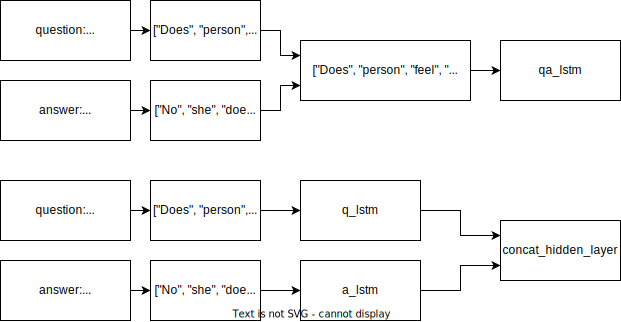
\includegraphics[width=.55\textwidth,keepaspectratio]{content/chapters/methodology/model_adaptation/figures/concat lstms vs q and a lstms.jpg}
    \captionsource(How Q and A are fed into the model){The difference in structure between the original (above) intended method --- where both question and answer are concatenated together --- and the final (below) method --- where the question and answer are passed into separate \glspl{lstm}.}{Original diagram prepared for this dissertation}
\end{figure}

%  Add a diagram explaining the changes made (such as a before and after).
% It needs to clearly illustrate the difference in structure between the original and the new implementation.

% Explain the training process (loading of data, initialisation of model, splitting of question and answer into pairs, setting of 0 or 1 if answer is correct, etc.)


\clearpage
\section{Experiments}
\label{sec:experiments}

Several experiments were conducted on the model to evaluate its performance on \gls{vcr}.
The experiments were designed to test the models accuracy over the three main task types (Q\rightarrow{}A, QA\rightarrow{}R, Q\rightarrow{}AR) discussed in Section~\ref{subsec:vcr_dataset} using different word embedding approaches and input encoder configurations.
Combinations of task type, \gls{bilstm} configuration in the model input unit and input token embedding types (contextual and noncontextual) were chosen as experiments to target what factors improve performance and what task types see the biggest improvement in prediction accuracy.

An additional experiment was also conducted on QA\rightarrow{}R to determine how big an influence the input answers had on the predicted rationale, and whether using previously-predicted answers as input would result in a significant drop in accuracy.
To test this, the model was first trained to predict the correct answers in Q\rightarrow{}A mode, exporting the predicted answers to a prediction file.
Then a new model was trained in QA\rightarrow{}R mode, using the predicted correct answers instead of the true correct answers.

\subsection{Setup}
\label{subsec:experiment-setup}

The model was trained on a single machine node with up to two \acrshort{gpu} nodes to use, depending on the configuration used for each experiment.
Each model was trained using a configuration file that selected the hyper-parameters used and task type to be tested.
To keep track of the model training history, model checkpoints were taken during training after every predefined number of steps.
Training was performed up to the specified step count, after which the model was evaluated using each of the recorded checkpoints.
To avoid recording the performance of an overfit model, the model performance chosen was taken from the step with the highest accuracy and not the most recent step.

\subsection{Ablations}
\label{subsec:experiment-ablations}

A set of ablation experiments were developed as part of the main experiments to determine the accuracy contribution of various components of the model.
Namely, those experiments deciding embedding types and \gls{bilstm} configuration.

The ablation tested is the use of context-aware token embeddings over context-free token embeddings, and whether a higher embedding dimensionality contributes to improved performance or not.
For this, BERT was chosen as the sentence-level context-aware embedding, retaining the same embeddings published by \citeauthor{zellers_recognition_2019} alongside the \gls{vcr} dataset and their \gls{r2c} model\cite{zellers_recognition_2019}.
To test context-free embeddings, GLOVE is used since it is the same embedding scheme used by \gls{snmn} and \gls{n2nmn} in their training and evaluation.
As an additional measure in testing context-free embeddings, Word2Vec embeddings are used which are generated using a Continuous Bag-Of-Words model\cite{mikolov_we_2013}.
Two sets of Word2Vec embeddings are generated, one with 300-dimensional vectors to match the GLOVE dimensionality and one with 768-dimensional vectors to match the BERT vectors.
This will both determine how big an effect both vector dimensionality and sentence-level context have on accuracy.

Another ablation is the testing of how the model input unit encodes the input sentences.
Seeing as the original model was designed with only a single token sequence in mind, one \gls{bilstm} encodes the sequence, but since we have more than one sequence as input, multiple \glspl{bilstm} are needed to encode each sequence.
As an ablation, another experiment is conducted where the model uses a single \gls{bilstm} to encode all three sequences.
This evaluates whether a single \gls{bilstm} would bottleneck the layout generation or improve it.

